\documentclass{standalone}
\usepackage{standalone}

\begin{document}
\chapter{Background Study}
\section{Literature Review}
In our study we found a few amount of academic approved papers related to our task personality prediction. Since the increasing information available on social networks, many authors interested in trying to predict user’s personality with the help of information people shared in Facebook.

Authors of [1] accurately measured the user personality through the public information available on their Facebook profiles along with 44 items and Big Five dimensions. Some of them are number of photos, features like relationship, date of birth, status, religion, education history, gender, home-town, personal activities etc. Authors tried to find the correlation between the data and Big Five Inventory and used profile data as feature and trained those data with two machine learning algorithm called m5sup/Rules and Gaussian Processes. Authors found a good result with RMSE error 0.73 for Openness, 0.73 for Conscientiousness, 0.99 for Extraversion, 0.73 for Agreeableness and 0.83 for Neuroticism.

Another work done on user personality prediction was described in [2]. Authors used both the Facebook user’s profile extracted data and also collected each data by Curiosity Exploration Inventory (CEI-II) form. For each user they collected total number of group they involved, total number of photos, total number of friends, total number of likes and some basic profile features like primary, high school and university (CEI-II) degree etc. Then they try to find correlation between the features and degree of curiosity. Finally they proposed a model with a decision tree with 3 searches and 8 evaluator methods. It is very important to notify that they used Weka3 an open source software to check performance their model. And showed that it is possible to predict a person’s curiosity with some specific features using J48 algorithm with a 10-cross-validation.

\begin{figure}[h]
				\centering
				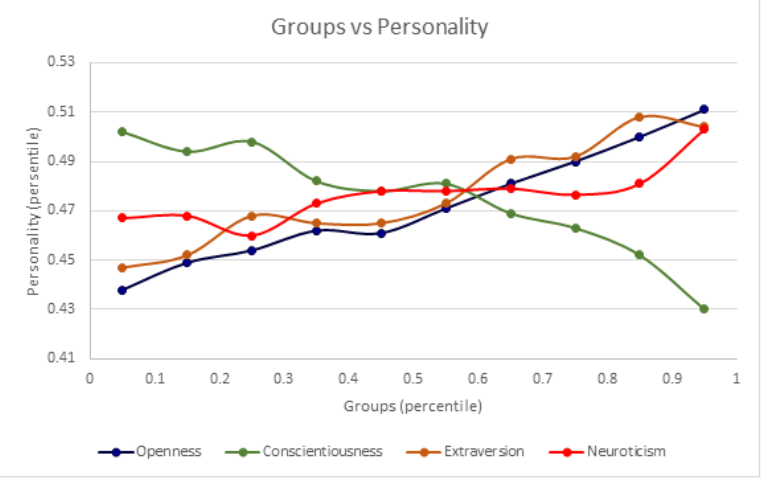
\includegraphics[scale=0.6]{./img/groupvsper}
				\caption{Groups vs Personality (percentile)} \label{fig:mapComp}
\end{figure}

In another work author extracted 1,80,000 user’s Facebook profile containing number of photos, number of groups, number of likes, size and density of friendships etc. Then tried to find correlation between their personality and profiles. It was showed that the best accuracy achieved for Extraversion and Neuroticism, the lowest accuracy achieved for Agreeableness and middle accuracy for Openness and Conscientiousness [Table: 2.1]. In their methodology they collected all Facebook features and they sorted the n users according to their number of friends feature for example from the user with the smallest number of Facebook friends to the user with the greatest number of Facebook friends, to obtain the sorted list u1, u2,....., un. They denote each user’s number of friends as ci. Then they partitioned those ordered users into k equal and disjoint sets. Where the set S1 of q = n/k users with the smallest number of friends), the following set S2 of q users with slightly higher feature values and so on until the set Sk contains q users of the highest feature values(users with the most friends). Authors partitioned users into k=10 large groups. Then they plotted Clustered Scatter Plots to show the relationship between Big Five Inventory Model and Facebook features where horizontal axis represented the average Facebook feature value and vertical axis represented the average personality trait score [Fig-2.1,2.2].

\begin{table}[h]
	\centering
	\begin{tabular}{|c|c|c|}
		\hline
		\begin{tabular}[c]{@{}c@{}}Trait\\ \end{tabular} & \begin{tabular}[c]{@{}c@{}}R^{2}\\ (\%)\end{tabular} & \begin{tabular}[c]{@{}c@{}}RMSE\\ (\%)\end{tabular} \\ \hline
		Openness & 0.11 & 0.29 \\ \hline
		Conscientiousness & 0.17 & 0.28 \\ \hline
		Extraversion & 0.33 & 0.27 \\ \hline
		Agreeableness & 0.01 & 0.29 \\ \hline
		Neuroticism & 0.26 & 0.28 \\ \hline
	\end{tabular}
	\caption{Predicting personality traits using Facebook features through multivariate linear regression}
	\label{tab:error5}
\end{table}

\begin{figure}[h]
				\centering
				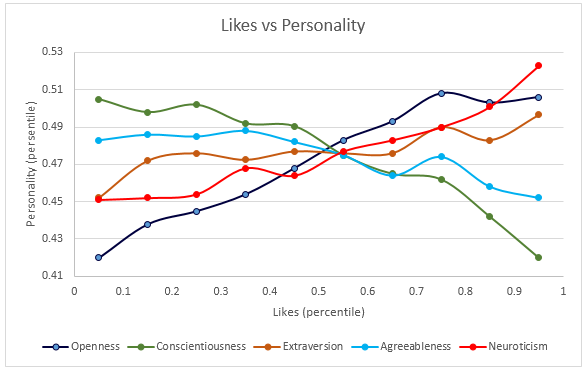
\includegraphics[scale=0.6]{./img/likevsper}
				\caption{Likes vs Personality (percentile)} \label{fig:mapComp}
\end{figure}

Another work described in [4]. Authors crawled 479k users profile data and analyzed based on three categories like gender, study that depicts the age distribution of users and inferred data from Facebook user’s profile. Mainly authors focused on the closed and disclosed section and measure degree of each Facebook user’s profile. Finally they showed that closed and disclosed section of users profile is depending on their age distribution [Fig-2.3] and gender distribution [Table-2.2].

\begin{figure}[h]
				\centering
				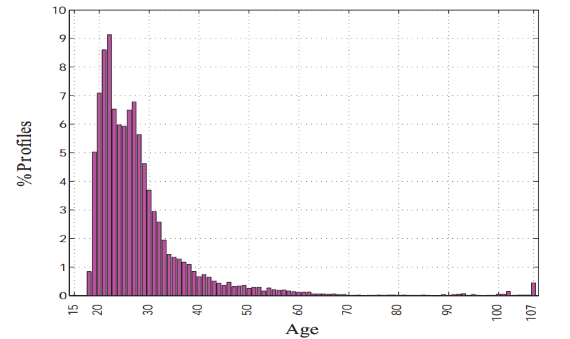
\includegraphics[scale=1.2]{./img/ager}
				\caption{\% Profiles in different age range} \label{fig:mapComp}
\end{figure}

\begin{table}[h]
	\centering
	\begin{tabular}{|c|c|c|}
		\hline
		\begin{tabular}[c]{@{}c@{}}Attributes categories\\ \end{tabular} & \begin{tabular}[c]{@{}c@{}}\%Male\\ (\%)\end{tabular} & \begin{tabular}[c]{@{}c@{}}\%Female\\ (\%)\end{tabular} \\ \hline
		All & 51.33 & 48.67 \\ \hline
		Friend-list & 53.99 & 46.01 \\ \hline
		CurrentCity & 52.81 & 47.19 \\ \hline
		HomeTown & 54.05 & 45.95 \\ \hline
		Gender & 51.33 & 48.67 \\ \hline
		Birthday & 49.23 & 50.77 \\ \hline
		Employers & 55.23 & 44.77 \\ \hline
		College & 53.30 & 46.70 \\ \hline
		HighSchool & 55.89 & 44.11 \\ \hline
	\end{tabular}
	\caption{Gender analysis per categories of attributes}
	\label{tab:error5}
\end{table}

Another work described in [5] authors collected users profile attributes, interests, advertising content users are exposed to is either relevant or irrelevant or not possible to explain based on their online activities [Table 2.3]. Then authors first applied Singular Value Decomposition (SVD) with k (user)-dimensional vector to build the model and used that model to for some unknown users to train.  

\begin{table}[h]
	\centering
	\begin{tabular}{|c|c|c|c|c|c|}
		\hline
		\begin{tabular}[c]{@{}c@{}}L#\\ \end{tabular} & \begin{tabular}[c]{@{}c@{}}Labels\\ \end{tabular} & \begin{tabular}[c]{@{}c@{}}Users(n)\\ \end{tabular}  & \begin{tabular}[c]{@{}c@{}}Balance\\ \end{tabular}  & \begin{tabular}[c]{@{}c@{}}m\\ \end{tabular}  & \begin{tabular}[c]{@{}c@{}}m^{'}\\ \end{tabular} \\ \hline
		L1 & Gay/Straight & 2412 & 50/50 & 218490 & 15609\\ \hline
		L2 & Single/Married & 7732 & 50/50 & 511775 & 29389\\ \hline
		L3 & Liberal/Conserv. & 4106 & 55/45 & 296298 & 18658 \\ \hline
		L4 & Muslim/Christian & 1196 & 74/26 & 134120 & 10333\\ \hline
	\end{tabular}
	\caption{Dataset overview}
	\label{tab:error5}
\end{table}

After analyzing authors focused on four target label pairs of sensitive nature a) gay vs straight, b) single vs married, c) liberal vs conservative and d) Christian vs Muslim. Then authors run feature selection process and removed those users that did not contain any of above label. Then authors showed that provide a clue that gay and straight can be performed more accurately than single and married.\\

In [6], authors tried to differentiate the relative influences of different feature extraction approaches like information retrieval feature (TFIDF),  document frequency (df), linguistic feature(lin), length of social snippet(lenText), relative position(pos) etc. on  social snippets and showed that TFIDF has most. Figure 2.4 shows their analysis.

\begin{figure}[h]
				\centering
				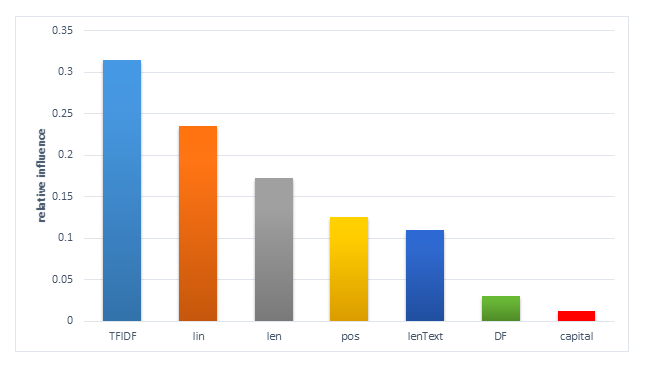
\includegraphics[scale=0.6]{./img/rref}
				\caption{The relative influence of each feature in Gradient Boosting Machine (GBM)} \label{fig:mapComp}
\end{figure}


\end{document}